\documentclass[a4paper,12pt, openany]{book}
\usepackage[subpreambles=true]{standalone}

%----------------------------------------
% LANGUE & TYPO
%----------------------------------------
\usepackage[french]{babel}
\usepackage{csquotes}
\usepackage{fontspec}
\usepackage{unicode-math}
\usepackage{microtype}

% Paragraphe : on garde l'indentation + un petit espace entre paragraphes
\setlength{\parindent}{20pt}
\setlength{\parskip}{0.8em}

% Couleurs (si besoin)
\usepackage{xcolor}

%----------------------------------------
% POLICES
%----------------------------------------
%\setmainfont{Times New Roman}
%\setmathfont{STIX Two Math}

% Désactive toutes les small caps (évite les warnings TU/.../sc)
%\makeatletter
%\DeclareRobustCommand{\textsc}[1]{#1}
%\renewcommand{\scshape}{\upshape}
%\makeatother

%----------------------------------------
% MISE EN PAGE
%----------------------------------------
\usepackage{geometry}
\geometry{margin=2.5cm}

\usepackage{setspace}
\onehalfspacing % (si tu veux simple interligne : commente cette ligne)

\usepackage{titlesec}
\usepackage{fancyhdr}
\usepackage{ragged2e}
\justifying
\usepackage{indentfirst}

\usepackage{booktabs, array, multirow, tablefootnote}
\usepackage{caption}
\captionsetup{
  labelfont={bf},      % label en gras (pas de small caps)
  textfont={normal},
  format=hang,
  margin=12pt
}

\usepackage{float}
\usepackage{wrapfig}
\usepackage{placeins}
\usepackage{tikz}
\usepackage{tikz-3dplot}
\usetikzlibrary{positioning,arrows.meta}
\usepackage{xurl}
\usepackage{epigraph}
\usepackage{enumitem}
\usepackage{comment}
\usepackage{mwe} % à retirer si inutile

%----------------------------------------
% GRAPHISMES & LIENS
%----------------------------------------
\usepackage{graphicx}

%----------------------------------------
% BIBLIO
%----------------------------------------
\usepackage[
  backend=biber,
  style=apa
]{biblatex}
\addbibresource{../../ref.bib}

% Mise en forme biblio
\renewcommand*{\bibfont}{\normalsize}
\setlength\bibhang{1cm}
\setlength\bibitemsep{6pt}
\defbibheading{bibliography}{\raggedright \textbf{Références} \vspace{12pt}}

% Neutralise l'usage potentiel des small caps par biblatex (selon styles)
\AtBeginDocument{%
  \providecommand*{\mkbibnamefamily}[1]{#1}%
  \renewcommand*{\mkbibnamefamily}[1]{#1}% noms d'auteurs sans \textsc
}

%----------------------------------------
% DATE
%----------------------------------------
\usepackage[french]{datetime2}

%----------------------------------------
% HYPERREF EN DERNIER
%----------------------------------------
\usepackage[hidelinks]{hyperref}

%----------------------------------------
% PIEDS DE PAGE
%----------------------------------------
\pagestyle{fancy}
\fancyhf{}
\fancyfoot[C]{\thepage}
\renewcommand{\headrulewidth}{0pt}
\renewcommand{\footrulewidth}{0pt}

% Veuves/orphelines
\clubpenalty=100000
\widowpenalty=100000
\displaywidowpenalty=100000
\brokenpenalty=100000



\begin{document}





\paragraph{Voir \textcites{hirschman82, holbrook82}} n



Les émotions sont au cœur du quotidien, comme l'illustre l'ampleur de l'intérêt qui leur est porté, à toutes époques et dans tous domaines, du moins en occident. En effet, la réflexion autour des émotions commence au moins par les penseurs de la Grèce Antique \parencite{plamper15}. Pourtant, celles-ci ne sont étudié scientifiquement en Occident qu'à partir du XIX$^{eme}$ siècle avec \textcite{darwin1872} et \textcites{james1884, james1894} \parencite{marcus2000}. Auparavant, les émotions étaient le sujet des philosophes, des écrivains et des dramaturges ; les enseignements qu'ils en ont tirés proviennent de leur réflexion et de leurs observations de la nature humaine autour d'eux.  \textcite{elster98} décrit en détails les réflexions sur les émotions en philosophie et littérature avant que ce sujet ne passe aux mains des sciences cognitives et sociales. \par 

Dans la seconde moitié du XX$^{eme}$ siècle, les sciences sociales et la culture connaissent ce que Patricia Clough identifie comme un «\;tournant affectif\;» \parencite{clough07}. \textcite{hardt07} explique ce tournant par les avancées des luttes sociales telles que le féminisme qui ont ramené les émotions et le domaine de l'affectif en général au centre des discussions. Pour illustrer le lien entre le féminisme et l'affect, \textcite{hardt07} prend l'exemple du travail affectif (travail maternel, soin des proches, etc) qui est souvent attribué aux femmes et est de par sa nature, lié au domaine de l'affect. Les sciences sociales sont à la pointe de ce tournant mais s'en saisissent chacune différemment. \par 

Aristote est considéré comme le premier en Occident à analyser la psychologie humaine de manière systématique \parencite{kennedy91}. Ses conclusions reposent sur l'observation et l'intuition et demeurent pertinentes encore aujourd'hui. Les contributions de Aristote se concentrent principalement sur les facteurs déclenchant les émotions, parmi elles, deux sont particulièrement intéressantes : l'existence de facteurs cognitifs précédant les émotions et la dualité d'une émotion ressentie. \par 

Auparavant les émotions étaient considérées comme un état comparable à une maladie, une situation incontrôlable. Aristote aborde l'idée que les émotions dépendent en partie des croyances, les facteurs cognitifs, que nous avons envers l'objet de l'émotion. Lors de sa réflexion sur la colère, Aristote conclut que cette émotion provient d'une injure lorsque que celle-ci est émise par quelqu'un n'étant pas en position d'injurier. C'est-à-dire que les insultes d'un parti hiérarchiquement supérieur tel un souverain ne déclenche pas de colère à l'instar d'insultes provenant d'un pair ou d'un subalterne. Cela signifie que la colère venant d'une injure dépend de nos croyances envers l'émetteur de l'injure. Ainsi, les émotions ont une dimension cognitive et peuvent donc être influencées en modifiant cette dimension. Par exemple, si l'on convainc un individu que même son souverain lui doit le respect alors une injure déclenchera de la colère. Pour l'émotion de la colère Aristote insiste sur l'asymétrie de pouvoir entre les deux partis. Ce déséquilibre apporte en plus une dimension sociale aux émotions notamment sur les relations de pouvoir et de statuts que la sociologie moderne développe. \par 

La notion de valence dans les émotions, le plaisir ou la douleur qu'une émotion apporte et dans quelle intensité, est une des rares caractéristiques des émotions sur laquelle toutes les disciplines sont d'accords. Pour Aristote, qui aborde aussi la notion de valeur, cela n'est pas contradictoire avec la notion de dualité, c'est-à-dire que toute émotion apporte à la fois du plaisir et de la douleur. Dans le deuil, la perte d'un être cher apporte indéniablement de la tristesse et pourtant dans les souvenir de cette personne se trouve une certaine joie. A l'inverse, dans la joie existe la douleur liée à l'anticipation de la fin du moment. Cette notion de dualité renseigne sur l'ambiguïté voir l'ambivalence de certaines émotions. Le ressenti simultané de plusieurs émotions participe à cette confusion. Cette réflexion pose la question de la neutralité de certains ressentis et émotions. Est-ce l'absence de valence, quelque chose de ni positif ni négatif ? Ou bien la présence simultanée d'émotions positives et négatives ? Ces questions sont au cœur de l'analyse des sentiments en sciences informatiques et influence directement l'identification d'émotions. Plus concrètement, dans le contexte de JDMA, cette dualité se retrouve dans les commentaires emplis d'émotions négatives et dont les auteurs mentionnent tout de même de la reconnaissance envers les agents pour leur accueil et leur accompagnement ; au milieu d'une expérience négative se trouve du positif. \par 

D'après \textcite{elster98} l'avancée majeure suivante dans la compréhension des émotions provient des moralistes français des XVI et XVII$^{eme}$ siècles. Plutôt que de se concentrer sur les déclencheurs des émotions et leurs conséquences directes, comme le fit Aristote, les moralistes s'interrogent surtout sur les mécanismes cognitifs liant les différentes étapes de l'émotionnel entre elles. Comment les émotions peuvent générer d'autres émotions ou indirectement influencer le jugement de chacun. Pour illustrer cette distinction, \textcite{elster98} se concentre sur l'envie. Pour Aristote, l'envie motive à empêcher d'autres d'obtenir ce que l'on désir sans mécanisme intermédiaire, par exemple en le détruisant. Pour La Rochefoucauld, l'envie agit en nous faisant dévaluer l'objet de ce désir afin de ne plus le vouloir. Ici, le mécanisme intermédiaire de dévaluation est pris en compte. De plus, la conscience de ressentir de l'envie qui est socialement perçue comme une faiblesse morale génère de la honte. Ainsi la cognition d'une émotion peut en générer une autre. Pour autant la conscience d'une émotion n'est pas nécessaire, cette conclusion incite une réflexion largement poursuivie en sociologie sur la possibilité de ressentir une émotion qui pour laquelle il n'y a pas de mot. \par 

\textcite{elster98} décrit une deuxième contribution importante des moralistes portant sur l'aspect social des émotions. Le premier tenant de cet aspect initié particulièrement par La Rochefoucauld : la notion d'amour-propre comme motivation fondamentale de l'humanité. L'amour-propre, ici, est à la fois une préoccupation de l'estime de soi et une préoccupation de l'estime des autres. Ces deux préoccupations génèrent la déception et l'auto-déception. La fierté et l'orgueil sont toutes deux des auto-déceptions permettant d'ignorer nos propres faiblesses. Les moralistes attribuent la longévité de la civilisation à la volonté d'être estimé. Cette volonté peut d'ailleurs être comprise comme le désir d'être apprécié ou la peur d'être critiqué. La volonté de préserver son amour-propre est semblable au concept de soi en psychologie sociale, l'image qu'un individu a de soi-même à un instant donné. Similairement à l'amour-propre, pour préserver un concept de soi positif, il existe des mécanismes émotionnels, psychologiques et comportementaux puissants. \par 

La notion d'amour-propre comporte une certaine incohérence : elle inclue s'estimer soi-même et être estimé par ses pairs simultanément. Or s'estimer soi-même explicitement est un obstacle à l'estime des autres lorsque cela est perçu comme de la vanité. Toute vertu ne peut être valorisée par autrui que si elle est réalisée avec modestie. Cette incohérence aggrave la différence entre être et paraître et impose le recours à ce que les moralistes nomment le voile et le masque. Le voile pour cacher une émotion, le masque pour en laisser paraître une différente de celle ressentie. S'il semble évident aujourd'hui que l'émotion exprimée n'est pas forcément l'émotion ressentie, la raison expliquant la différence entre ce qui est exprimé et ce qui est ressenti ne l'est pas. Les moralistes apportent un premier élément de réponse : l'émotion exprimée est celle qui est socialement appropriée dans la situation, celle qui correspond aux normes.

\section{Classifications des émotions}
\subsection{Les émotions sont-elles universelles ?}
	
L'approche évolutionniste des émotions, initialement proposée par \textcite{darwin1872} est l'un des précurseur de l'étude des émotions telle qu'elle est menée aujourd'hui. Cette approche postule initialement que les émotions sont le produit d'une évolution génétique universelle à tous les êtres humains et aux animaux, du moins la plupart. \textcite{darwin1872} a interrogé des participants sur l'émotion communiquée par l'expression faciale d'un acteur au travers d'un questionnaire envoyé au quatre coins du monde. Les résultats de ce questionnaire combinés avec ses observations l'amènent à la conclusion de l'universalité des émotions due aux similarités de leur expression à travers plusieurs cultures. Notamment, Darwin identifie six émotions principales : colère, peur, surprise, dégoût, joie et tristesse. \par


Soutenir que les émotions sont universelles ne signifie pas que toutes les émotions le sont. 
La question d'émotion basique est récurrente parmi les chercheurs. Théoriquement une émotion basique est une émotion universelle, c'est-à-dire présente chez tout le monde et c'est une émotion non pas apprise mais innée et donc causée par des facteurs biologiques. Par exemple l'approche de \textcite{ekman71} identifie six émotions basiques car elles se manifesteraient de manière similaire sur le visage des membres de plusieurs tribus et cultures différentes indépendamment de la langue. Ces six émotions sont : la joie, la tristesse, la colère, la peur le dégout et la surprise. Cette liste a été étendue plusieurs fois au fur et à mesure \parencites{ekman92a, ekman99}. Il existe plusieurs listes suggérées de ces émotions basiques comme le montre le tableau~\ref{tab:basiques}, celles-ci peuvent varier significativement d'une liste à l'autre. Cependant, la majorité des chercheurs sont d'accord sur l'inclusion de la colère, la joie, la tristesse et la peur et de nombreuses différence proviennent de l'utilisation mots quasi synonyme pour décrire la même émotion par exemple colère et rage ou attente, anticipation et désire \parencite{ortony90}.  Les défendeurs de l'existence d'émotions basiques donnent plusieurs arguments. Certaines émotions seraient exprimées sur les visages de plusieurs cultures très diverses de manière similaire permettant une certaine compréhension \parencite{ekman92b}. \textcite{plutchik62} défend l'existence de huit émotions basiques couplées en opposées : La colère et la peur, la joie et la tristesse, la confiance et le dégout, l'anticipation et la surprise. Ces émotions sont choisies car elles conduisent toutes à un comportement bénéfique à la survie, la colère pousse à se battre, la peur à fuir, le dégout à éviter, la confiance à la coopération etc. De plus, ces émotions se retrouvent chez de nombreuses espèces animales, cela renforce la théorie que ces émotions sont basiques et universelles. Plus récemment, des avancées en sciences cognitives montrent que certaines émotions activent systématiquement les mêmes zones du cerveau \parencite{celeghin17}. \par  

\begin{table}[!ht]
    \centering

    \caption{Sélection de listes d'émotions « basiques »}
    \label{tab:basiques}    
    \begin{tabular}{p{4cm} p{7cm} p{4.3cm}}
        \hline
        \textbf{Référence} & \textbf{Émotions basiques} & \textbf{Critères d'inclusion} \\
        \hline
	    \textcite{arnold60} & \raggedright Colère, aversion, courage, découragement, désir, désespoir, peur, haine, espoir, amour, tristesse & \raggedright Relation aux tendances d'action \tabularnewline
        \textcite{darwin1872} & Colère, peur, surprise, dégoût, tristesse & Expressions faciales universelles \\
       \raggedright \textcite{ekman82} & \raggedright Colère, dégoût, peur, joie, tristesse, surprise & \raggedright Expressions faciales universelles \tabularnewline
        &&\\
      \raggedright  Frijda (communication personnelle, 8 septembre 1986) & \raggedright Désir, bonheur, intérêt, surprise, émerveillement, chagrin & \raggedright Formes de préparation à l'action \tabularnewline
        &&\\
        \raggedright \textcite{gray84} & \raggedright Rage et terreur, anxiété, joie & \raggedright Inhérent \tabularnewline
        &&\\
        \raggedright \textcite{izard71} & \raggedright Colère, mépris, dégoût, détresse, peur, culpabilité, intérêt, joie, honte, surprise & \raggedright Inhérent \tabularnewline
        &&\\
        \raggedright \textcite{james1884} & \raggedright Peur, tristesse, amour, rage & \raggedright Implication corporelle \tabularnewline
        &&\\
        \raggedright \textcite{mcdougall26} & \raggedright Colère, dégoût, exaltation, peur, soumission, tendresse, émerveillement & \raggedright Relation aux instincts \tabularnewline
        &&\\
       \raggedright \textcite{mowrer60} & \raggedright Douleur, plaisir & \raggedright États émotionnels innés \tabularnewline
        &&\\
        \raggedright \textcite{oatley87} & \raggedright Colère, dégoût, anxiété, bonheur, tristesse & \raggedright Ne nécessitent pas de contenu propositionnel \tabularnewline
        &&\\
        \raggedright \textcite{panksepp82} & \raggedright Attente, peur, rage, panique & \raggedright Inhérent \tabularnewline
        &&\\
        \raggedright \textcite{plutchik80a} & \raggedright Acceptation, colère, anticipation, dégoût, joie, peur, tristesse, surprise & \raggedright Relation aux processus biologiques adaptatifs \tabularnewline
        &&\\
        \raggedright \textcite{tomkins84} & \raggedright Colère, intérêt, mépris, dégoût, détresse, peur, joie, honte, surprise & \raggedright Densité du déclenchement neuronal \tabularnewline
        &&\\
        \raggedright \textcite{watson30} & \raggedright Peur, amour, rage & \raggedright Inhérent \tabularnewline
        &&\\
        \raggedright \textcite{weiner84} & \raggedright Bonheur, tristesse & \raggedright Indépendant de l'attribution \tabularnewline
        \hline

    \end{tabular}
	\caption*{\small \textit{Note :} Tableau provenant de \textcite{ortony90} et complété.}
\end{table}


Pour certains chercheurs, les émotions basiques représentent aussi les fondations de toutes émotions, c'est-à-dire que toute émotion peut être définie en terme d'émotions basiques. Ce raisonnement est similaire à l'analyse des couleurs qui se basent sur des couleurs primaires, irréductible et composant toute autre couleur. Par exemple, pour \textcite{kemper87}, qui considère la peur, la colère, la dépression et la satisfaction comme les quatre émotions basiques, la culpabilité est une émotion produite par le déclenchement de peur bien que la culpabilité est une émotion apprise au travers d'interactions sociales. En revanche, pour \textcite{plutchik80}, les mélanges d'émotions basiques créent de nouvelles émotions plus complexes ; l'amour proviendrait du mélange entre joie et confiance, deux émotions que Plutchik considère comme basiques (voir figure~\ref{fig:wheel}). \par 


À l'inverse, les opposants à la théorie d'émotions basiques, tout d'abord, remarquent que le manque de consensus sur la liste des émotions basiques décrédibilise la théorie ; ce que certains considèrent comme des émotions basiques, d'autres ne considèrent pas du tout comme une émotion telle que la surprise \parencite{ortony90}. Aristote identifiait 15 émotions basiques, Descartes 6, Hume seulement 2, 3 pour Spinoza etc \parencite{thamm06}. \textcite{ortony90} suggèrent que ce désaccord sur la liste des émotions basiques provient du fait que ce ne sont pas des émotions qui sont basiques mais des éléments fondateurs des émotions. Dans le cas de la surprise, ces auteurs estiment que la surprise n'est pas une émotions car elle n'a pas de valence propre, une surprise peut être positive, négative ou neutre. Cependant, la surprise est un critère pour d'autres émotions comme le choque. Ainsi la surprise ne serait pas une émotion basique mais la présence ou non de surprise serait un paramètre fondateur des émotions. \par 

\begin{figure}[!ht]
\centering
\caption{Roue des émotions de Plutchik (1962)}
\label{fig:wheel}
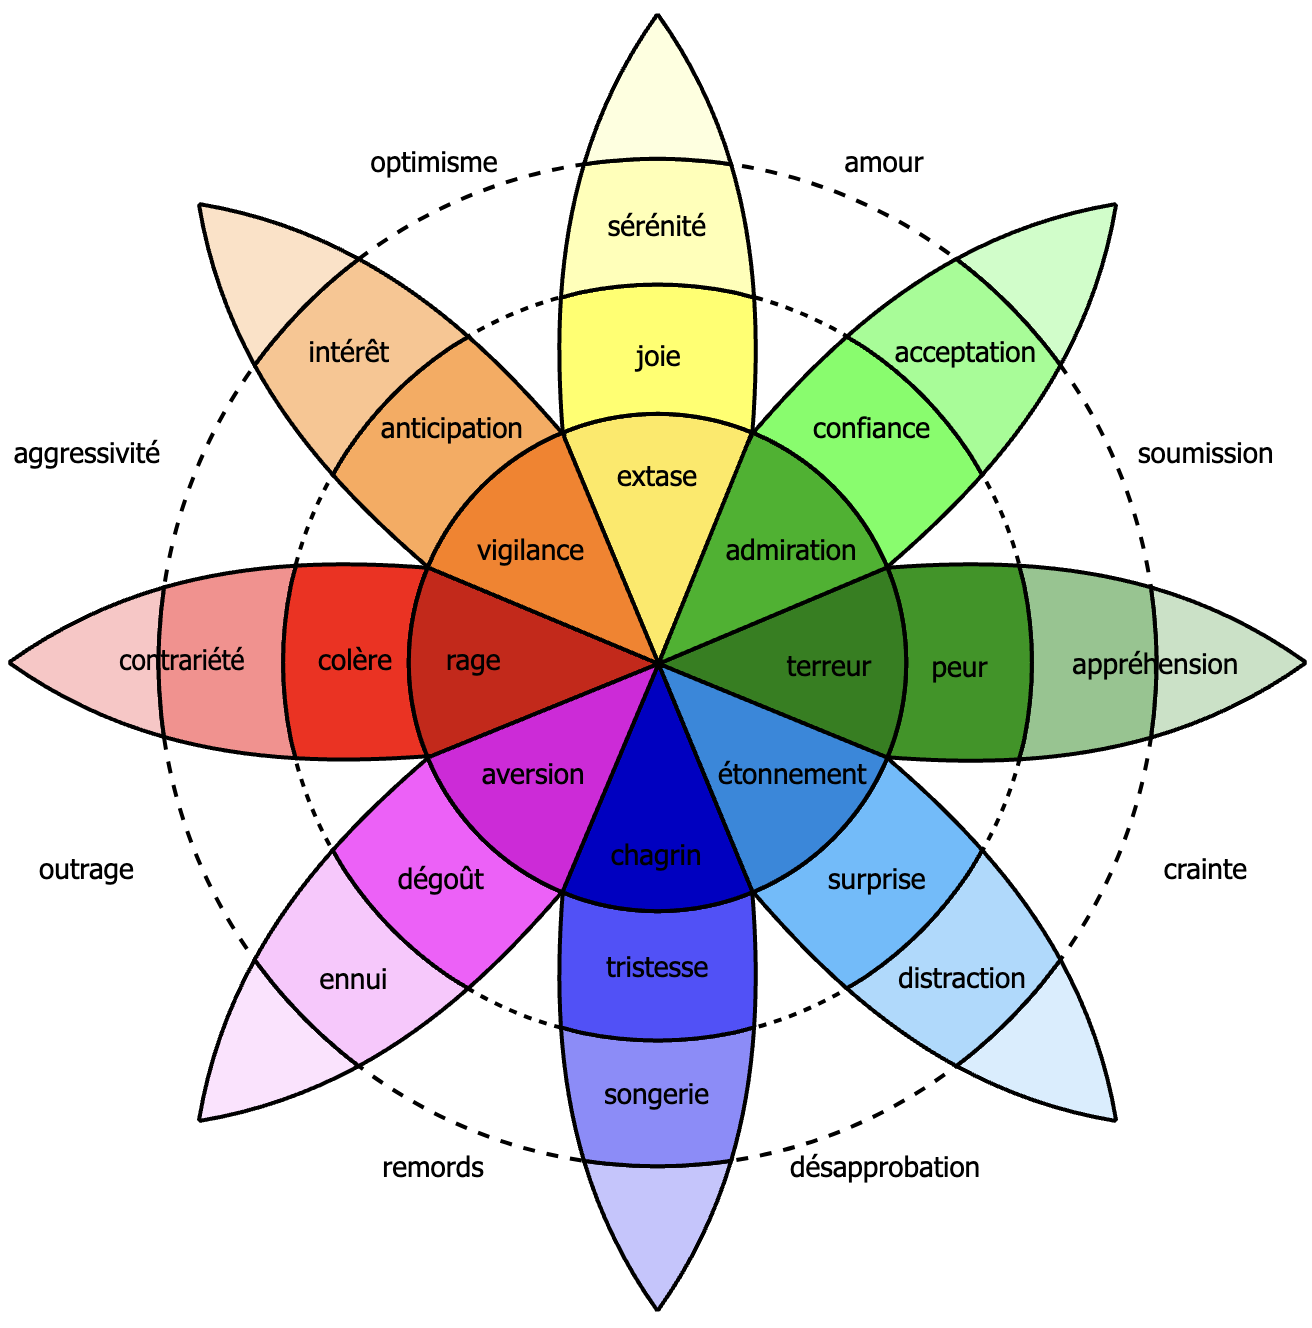
\includegraphics[width=0.575\linewidth]{Images/Plutchik_wheel.png}
\end{figure}

De plus, les opposants à la théorie d'émotions basiques reprochent à ce concept d'ignorer l'importance de la culture \parencites{barrett06, barrett12}, de minimiser les différences culturelles \parencite{mesquita92, mesquita16} et de confondre la distinction entre le mot et le concept. Par exemple le mot «colère» n'est pas forcément assigné au même sentiment de colère pour chacun \parencite{ortony22}. Il existe un composant social aux émotions, pour le justifier \textcite{barrett12} propose un raisonnement en deux étapes. Premièrement, l'idée qu'il n'y a pas de correspondance entre une émotion et une réaction physique ou cognitive, c'est-à-dire que la même réaction physique (changement de rythme cardiaque, transpiration, activation de neurones…) peut être catégorisée comme différentes émotions par différentes personnes, ainsi une émotion ne peut pas être définie par un changement corporel seulement. Deuxièmement, cette catégorisation d'une réaction physique et cognitive est générée par un accord social entre membres d'une même société. Prenons pour exemple un patient et son thérapeute, le patient peut relater un évènement difficile, telle que la perte d'un proche, provoquant chez lui de la colère et le thérapeute l'interpréter comme de la tristesse, dans cette situation aucun des deux n'aurait tort ou raison puisque qu'il n'y a pas de vérité objective et mesurable. Le patient a réellement ressenti quelque chose qu'il catégorise comme de la colère et le thérapeute a réellement perçu quelque chose qu'il catégorise comme de la tristesse. Les catégorisations de chacun dépendent de comment ils identifient la colère et la tristesse. Or cette identification dépend des normes sociales et culturelles les entourant. Par conséquent, les émotions que nous ressentons sont influencées par notre culture et notre société. \par 


\break

	\subsection{Comment classifier les émotions ?}
	
Lorsque l'on tente de définir et comprendre ce que sont les émotions, on en vient forcément à se demander si elles sont liées et comment. Il existe deux approches principales pour organiser et classifier les émotions : l'approche par labellisation et l'approche par dimensions structurelles. La première approche considère les émotions comme des catégories discrètes et tente de toutes les recenser et de les classifier comme les éléments dans le tableau périodique ou les plantes dans un herbier. La deuxième approche tente d'identifier les dimensions qui structurent chaque émotion ; en d'autres mots, les facteurs par lesquels toute émotion peut être résumée. \par 



		\subsubsection{Classification par labellisation}

La classification par labellisation imagine les émotions comme des catégories propres chacune définissable. Ces catégories peuvent avoir des points communs : la joie et la fierté sont toutes les deux des émotions plaisantes, elles ne sont pas forcément contradictoires non plus, elles peuvent être ressenties simultanément mais elles sont bel et bien différentes. Les premiers partisans de cette approche ont commencé par une labellisation classique, c'est-à-dire que pour être classifier comme appartenant à une émotion, un ressenti devait remplir des conditions «\;nécessaires et suffisantes\;» \parencite{clore88}. Cette façon de faire est critiquée notamment par \textcite{russell91} car aucune liste de conditions pour chaque émotion n'a jamais fait consensus après des siècles de tentatives. \textcite{russell91} défend plutôt une méthode prototypique qui prendrait en compte non pas les caractéristiques nécessaires mais celles du cas typique, par exemple remplir les caractéristiques typique de la colère pour être catégorisé comme tel, même s'il existe des exceptions. \par 


		\subsubsection{Classification dimensionnelle}	

Les émotions sont aussi souvent classées selon leurs dimensions fondatrices. La classification dimensionnelle considère les émotions n'ont pas comme des catégories distinctes mais comme les résultats de combinaisons spécifiques de dimensions sous-jacentes. Ces dimensions sont des axes sur lesquels peuvent être placées les émotions. Par exemple la dimension de la valence est fréquemment utilisée, c'est-à-dire si elles sont positives ou négatives. Ces dimensions ne sont pas binaires ; la joie et la fierté sont toutes deux des émotions à valence positive mais la joie est généralement plus positive que la fierté. Il va de soi que la valence seule ne suffit pas à définir distinctement toutes les émotions, d'autres dimensions sont nécessaires. C'est là que se concentre la réflexion de la classification dimensionnelle. Cette réflexion n'est pas nouvelle et provient de la philosophie, par exemple \textcite{spinoza1677} soutient implicitement l'existence de deux dimensions : de joie à tristesse et pour le désir d'absence à présence. L'un des avantages de cette classification est que les émotions peuvent être représentées visuellement telle des coordonnées sur un graphique cartésien. \par 

Une classification dimensionnelle est appelée un modèle. Son objectif est de trouver les dimensions nécessaires à la qualification de chaque émotion avec le moins de chevauchement possible des dimensions entre-elles. Il s'agit de trouver l'équilibre entre pas assez de dimensions ce qui ne permet pas d'expliquer toutes les émotions et entre trop de dimensions qui seraient trop similaires tout en complexifiant une analyse. Chaque modèle se distingue des autres le plus souvent soit par la quantité de dimensions prises en compte soit par la nature des dimensions identifiées. La plupart des modèles se limitent à deux ou trois dimensions, par exemple \textcite{wundt1897} identifie les dimensions absence ou présence de plaisir, excitation ou calme, tension ou relaxation. Cette limitation à deux ou trois dimensions s'explique d'abord par la difficulté de représenter visuellement et de comprendre un modèle avec plus de trois dimensions et ensuite par une convergence d'études psychométriques trouvant deux ou trois dimensions selon les spécificités de l'étude \parencites{osgood66, schlosberg54, abelson62, gladstones62, williams65}. Il existe tout de même quelques exceptions comme \textcite{fontaine07} qui trouvent quatre dimensions : valence, contrôle (sur l'émotion), activation, imprévisibilité. \par


Aujourd'hui, les deux modèles les plus utilisés \parencite{wang22} sont \textit{le modèle circumplexe de l'affect} (\textcite{russell80} voir figure~\ref{fig:circumplex}) et le \textit{modèle des états émotionnels PAD} (\textcite{mehrabian74} voir figure~\ref{fig:pad} avec des exemples d'émotions) ; PAD signifie Plaisir Activation (excitation) Dominance. Le modèle circumplexe décrit les émotions sur deux dimensions : la valence de positif à négatif et l'activation de haute excitation à basse excitation au sein d'un cercle, chaque arc-de-cercle appartient à une émotion. Ainsi, en décrivant à quel point l'un est activé et ce qu'il ressent est positif ou négatif, il est possible d'approximer l'émotion ressentie. Le modèle PAD se distingue en ajoutant une dimension : la dominance ou soumission. Avec ce modèle, on doit pouvoir représenter toutes les émotions sur trois axes au lieu de deux dans le modèle circumplexe. Le troisième axe : dominance - soumission permet par exemple de distinguer la colère de la peur ; en colère nous nous sentons en contrôle de la situation, apeuré nous nous sentons acculés, sans issue. \par 

\begin{figure}[!ht]
\centering
\caption{Modèle circumplexe des émotions \parencite{russell99}}
\label{fig:circumplex}
\begin{tikzpicture}[scale=5, font=\footnotesize]

  % Draw main axes
  \draw[->, thick] (0,-1.1) -- (0,1.1) node[above=2pt, font=\bfseries] {Activation};
  \draw[->, thick] (-1.1,0) -- (1.1,0) node[right=2pt, font=\bfseries] {Agréable};
  \node[below=2pt, font=\bfseries] at (0,-1.1) {Désactivation};
  \node[left=2pt, font=\bfseries] at (-1.1,0) {Désagréable};

  % Circle boundary
  \draw[thick] (0,0) circle(1);

  % Emotion points (inner ring)
  \foreach \angle/\radius/\label in {
    110/0.82/tendu,
    120/0.72/nerveux,
    135/0.66/stressé,
    150/0.6/contrarié,
    200/0.65/triste,
    220/0.7/déprimé,
    240/0.75/léthargique,
    255/0.8/fatigué,
    285/0.8/calme,
    300/0.75/détendu,
    320/0.7/serein,
    340/0.65/content,
    20/0.65/heureux,
    40/0.7/élancé,
    60/0.75/excité,
    80/0.82/alerte}
    \node at ({\angle}:\radius) {\label};

  % Category labels (outer ring, bold, no overlap)
  \foreach \angle/\radius/\text in {
    90/1.27/Surprise,
    115/1.22/Peur,
    140/1.22/Colère,
    165/1.22/Dégoût,
    225/1.22/Léthargie,
    195/1.27/Tristesse,
    315/1.22/Détente,
    10/1.22/Bonheur,
    45/1.22/Excitation
    }
    \node[font=\bfseries] at ({\angle}:\radius) {\text};

\end{tikzpicture}
\end{figure}

\break

\begin{figure}[t]
\centering
\caption{Modèle dimensionnel PAD des émotions, avec quelques catégories émotionnelles, traduit de \textcite{lance10}.}
\label{fig:pad}
\tdplotsetmaincoords{75}{125} % viewing angle
\begin{tikzpicture}[scale=4,tdplot_main_coords]

  % Define cube dimensions
  \def\N{2}

  % Draw the cube
  \foreach \x in {0,0,\N}
    \foreach \y in {0,0,\N}
      \draw[gray!70] (\x,\y,0) -- (\x,\y,\N); % vertical lines

  \foreach \x in {0,0,\N}
    \foreach \z in {0,0,\N}
      \draw[gray!70] (\x,0,\z) -- (\x,\N,\z); % front-back lines

  \foreach \y in {0,0,\N}
    \foreach \z in {0,0,\N}
      \draw[gray!70] (0,\y,\z) -- (\N,\y,\z); % left-right lines

  % Shade the right side
  \fill[gray!20,opacity=0.6] (\N,0,0) -- (\N,\N,0) -- (\N,\N,\N) -- (\N,0,\N) -- cycle;

  % Axis labels
  \draw[->,thick] (0,0,0) -- (\N+0.5,0,0) node[anchor=north west]{\textbf{Dominance}};
  \draw[->,thick] (0,0,0) -- (0,\N+0.5,0)
  node[anchor=south east, xshift=15pt, yshift=7pt, font=\bfseries] {Plaisir};
  \draw[->,thick] (0,0,0) -- (0,0,\N+0.5) node[anchor=south]{\textbf{Activation}};

  % Emotion points and labels (with anchor dots)
\filldraw[black] (2,2,2) circle (0.8pt);
\node[anchor=south] at (2,2.5,2.1) {Excitation};

\filldraw[black] (2,0,2) circle (0.8pt);
\node[anchor=south east] at (2,0,2) {Colère};

\filldraw[black] (0,0,2) circle (0.8pt);
\node[anchor=south west] at (0,0,2) {Peur};

\filldraw[black] (2,0,0) circle (0.8pt);
\node[anchor=north east] at (2,0,0.2) {Mépris};

\filldraw[black] (0,0,0) circle (0.8pt);
\node[anchor=north west] at (0,0.1,0.2) {Tristesse};

\end{tikzpicture}
\end{figure}

\section{Théorie du pouvoir et du statut}

\section{Théorie dramaturgique}
\subsection{L'expression des émotions : le rôle que l'on se donne}




\end{document}